	\documentclass[10pt,oneside]{CBFT_book}
	% Algunos paquetes
	\usepackage{amssymb}
	\usepackage{amsmath}
	\usepackage{graphicx}
% 	\usepackage{libertine}
% 	\usepackage[bold-style=TeX]{unicode-math}
	\usepackage{lipsum}

	\usepackage{natbib}
	\setcitestyle{square}

	\usepackage{polyglossia}
	\setdefaultlanguage{spanish}
	



	\usepackage{CBFT.estilo} % Cargo la hoja de estilo

	% Tipografías
	% \setromanfont[Mapping=tex-text]{Linux Libertine O}
	% \setsansfont[Mapping=tex-text]{DejaVu Sans}
	% \setmonofont[Mapping=tex-text]{DejaVu Sans Mono}

	%===================================================================
	%	DOCUMENTO PROPIAMENTE DICHO
	%===================================================================

\begin{document}

% 
% =================================================================================================
\chapter{El oscilador armónico}
% =================================================================================================

Clásicamente la cosa venía de una partícula sometida a un potencial
\[
	V(x) = \frac{kx^2}{2} \qquad \qquad \omega = \sqrt{\frac{k}{m}}.
\]

Para el oscilador armónico cuántico 1D el hamiltoniano y energía son
\[
	H = \frac{p^2}{2m} + \frac{m\omega^2 x^2}{2} \qquad E = \hbar \omega \left( n + \frac{1}{2} \right)
\]
donde $\omega^2$ es la constante del resorte cuántico.
Este problema puede resolverse usando un nuevo operador $\hat{a}$ (operadores de aniquilación
y creación)
\[
	\hat{a} = \sqrt{\frac{m\omega}{2\hbar}}\left( x + i\frac{p}{m\omega} \right) \qquad \text{con} \quad 
	\hat{a}^\dagger = \sqrt{\frac{m\omega}{2\hbar}}\left( x - i\frac{p}{m\omega} \right)
\]
que es suma de $\hat{x}, \hat{p}$ pero que no es hermítico. Cumple que 
\[
	[a , a^\dagger ] = 1 \qquad a a^\dagger =  \frac{H}{\hbar\omega} -1 \qquad 
	H = \hbar\omega \left( a a^\dagger + \frac{1}{2} \right),
\]
donde se define el operador número $\hat{N}\equiv a^\dagger a$ que al verificar $[\hat{N},\hat{H}]=0$ tienen 
base de 
autoestados en común $\{ \Ket{n} \}$. En efecto 
\[
	\hat{N} \Ket{n} = n\Ket{n} \qquad
	\hat{H} \Ket{n} = \hbar\omega \left( n + \frac{1}{2} \right) \Ket{n}
\]
siendo $n$ el número de cuantos de energía.
Se cumplen además 
\[
	[N,a] = [a^\dagger a,a] = - [ a, a^\dagger a ] = - \left( a^\dagger [a,a] + [a,a^\dagger]a \right) =
	-a
\]
\[
	[N,a^\dagger] = [a^\dagger a, a^\dagger ] = - [a^\dagger , a^\dagger a ] =
	- \left( a^\dagger [a^\dagger,a] + [a^\dagger,a]a^\dagger \right) = a^\dagger
\]

Queremos ver que le  hace $a^\dagger$  a un autoestado $\Ket{n}$ y luego $a$ sobre el mismo.
\[
	N a^\dagger \Ket{n} = ([N, a^\dagger] + a^\dagger N) \Ket{n} =
	a^\dagger \Ket{n} + a^\dagger n \Ket{n} 
\]
\[
	\Hat{N} (a^\dagger\Ket{n}) = (n+1)(a^\dagger\Ket{n})
\]
Entonces, como no hay degeneración y tenemos $N\Ket{n'} = n'\Ket{n'}$ entonces 
\[
	a^\dagger \Ket{n} = c_1 \Ket{n+1},
\]
y procediendo de modo idem para $a\ket{n}$ será
\[
	a \Ket{n} = c_2 \Ket{n-1}
\]
Luego,
\[
	a^\dagger \Ket{n} = c_1 \Ket{n+1} \overbrace{\longrightarrow}^{DC} 
	\Bra{n+1} c_1^* = \Bra{n} a 
\]
\[
	a \Ket{n} = c_2 \Ket{n-1} \overbrace{\longrightarrow}^{DC} \Bra{n-1} c_2^* = \Bra{n} a^\dagger
\]
y entonces 
\[
	\Braket{n|N|n} = n \Braket{n|n} = n =  \Braket{n| a^\dagger a |n} =  \Braket{n-1|c_2^* c_2|n-1} =
	|c_2|^2 \Braket{n-1|n-1}
\]
\[
	n = \Braket{n|aa^\dagger-1|n} = -1 + \Braket{n|aa^\dagger|n} = - 1 + \Braket{n+1|c_1^*c_1|n+1} =
	-1 + |c_1|^2 \Braket{n+1|n+1}
\]
siendo
\[
	|c_2| = \sqrt{n} \qquad |c_1| = \sqrt{n+1} 
\]
\[
	\hat{a}^\dagger \Ket{n} = \sqrt{n+1} \Ket{n+1} \qquad  \hat{a}\Ket{n} = \sqrt{n} \Ket{n-1} 
\]
y entonces de esta forma $\hat{a}^\dagger$ es el operador de creación de cuantos y $\hat{a}$ el de 
aniquilación.
Estos operadores permiten ir saltando de niveles de energía y pasar entre estados definidos estos
por el número de cuantos.
Nótese que $\hat{a}$ es operador de aniquilación cuando actúa sobre kets; sobre bras los crea.

Del producto interno se tiene
\[
	(\Bra{n}a^\dagger)(a\Ket{n}) \geq 0
\]
lo cual conduce a $ n \geq 0 $.

\subsection{El estado fundamental $\Braket{0}$}

\[
	a \Ket{n}  \overbrace{\longrightarrow}^{DC} \Bra{n} a^\dagger
\]
y desde el postulado para productos internos,
\[
	(\Bra{n}a^\dagger)(a\Ket{n}) \geq 0 \quad n \Braket{n|n} \geq 0 \Rightarrow n \geq 0 
\]
entonces $n$ cabalga por los naturales.
Si hacemos 
\[
	a\Ket{n} = \sqrt{n} \Ket{n-1}, \quad  
	a^2 \Ket{n} = \sqrt{n (n-1)} \Ket{n-2} \quad 
	a a^2 \Ket{n} = \sqrt{n (n-1)(n-2)} \Ket{n-3} \; ...
\]
en algún momento (dado que $n\geq 0$) se llega a $\Ket{n=0}$, entonces $E_0 = \hbar\omega/2$ y 
\[
	\Ket{0} \equiv \text{El fundamental}
\]
y no se puede bajar más,
\[
	\hat{a}\Ket{0} = 0.
\]

Por otra parte, con el $\hat{a}^\dagger$ se puede llegar a cualquier estado
\[
	a^\dagger \Ket{0} = \sqrt{1} \Ket{1}, \qquad  a^{\dagger 2} \Ket{0} = \sqrt{1}\sqrt{2} \Ket{2} = 
	\sqrt{1}\sqrt{2}\sqrt{3} \Ket{3}
\]

\begin{figure}[htb]
	\begin{center}
	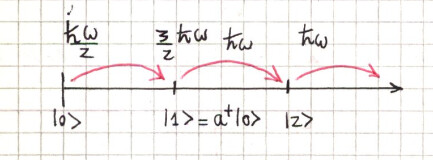
\includegraphics[width=0.6\textwidth]{images/fig_ft2_osc_arm1.jpg}	 
	\end{center}
	\caption{}
\end{figure} 

Se tienen todos los valores de energía a partir de uno solo,
\[
	\frac{{(a^{\dagger})}^n}{\sqrt{n}!} \Ket{0} = \Ket{n} \qquad \qquad 
	E_n = \hbar \omega \left( n + \frac{1}{2} \right)
\]

Las matrices de $\hat{a},\hat{a}^\dagger$ sólo tienen una diagonal corrida de elementoss 
\[
	\Braket{n'|a|n} = \sqrt{n} \Braket{n'|n-1} = \sqrt{n} \delta_{n',n-1}
\]
\[
	\Braket{n'|a^\dagger|n} =  \sqrt{n-1} \Braket{n'|n+1} = \sqrt{n-1} \delta_{n',n+1}
\]
Es decir, que pictóricamente serían algo como
\[
	a^\dagger = \begin{pmatrix}
	0 & \sqrt{1} & 0 & 0 & ... \\
	0 & 	0    & \sqrt{2} & 0 & ... \\
	0 & 	0    & 0 & \sqrt{3} & ... \\
	0 & ... \\
	0 & ... & & & \sqrt{n} \\
	0 & ... & & & 0 
	\end{pmatrix}
\]
y
\[
	a = \begin{pmatrix}
	0 & 0 & & & \\
	\sqrt{1} & 0 & 0 & & ... \\
		0    & \sqrt{2} & 0 & & ... \\
	 	0    & 0 & \sqrt{3} & &... \\
	 ... \\
	 ... & & & \sqrt{n} & 0 \\
	\end{pmatrix}
\]
Los elementos de las matrices
\[
	\Braket{n'|x|n} = \sqrt{\frac{\hbar}{2m\omega}}
	(\sqrt{n}\delta_{n',n-1} + \sqrt{n+1}\delta_{n',n+1})
\]
\[
	\Braket{n'|p|n} = i \sqrt{\frac{\hbar}{2m\omega}}
	(-\sqrt{n}\delta_{n',n-1} + \sqrt{n+1}\delta_{n',n+1})
\]
no pueden ser matrices diagonales porque no conmutan con el hamiltoniano.

También puede verse que 
\[
	\vm{x} = \Braket{n|x|n}= 0 \qquad \vm{p} = \Braket{n|p|n}= 0,
\]
lo cual difiere de lo que esperaríamos clásicamente. Es más, se tienen también
\be
	x^2 = \frac{\hbar}{2 m \omega}( a^2 + a^{\dagger 2} + aa^\dagger + a^\dagger a )
	\label{x2_osc_arm}
\ee
y consecuentemente
\[
	\Braket{0|x^2|0}= \frac{\hbar}{2 m \omega} \qquad 
	\Braket{0|p^2|0}= \frac{\hbar m \omega}{2}
\]
de manera que resulta
\[
	\Braket{(\Delta x)^2}_{\Ket{0}} \Braket{(\Delta p)^2}_{\Ket{0}} = \frac{\hbar^2}{4} 
\]
el estado fundamental es el de incerteza mínima.
Esto es así porque estamos en el fundamental y es un pack gaussiano.

Veamos ahora la forma que tiene la función de onda. A tiempo cero.
Siendo $\Psi_n(x') = \Braket{x'|n}$ quiero evaluar $\Psi_0(x') = \Braket{x'|0}$ y ver que como 
\[
	\Braket{x'|a|0}= 0 
\]
tengo 
\[
	0 = \sqrt{ \frac{m\omega}{2\hbar} } \Braket{x'|x+\frac{ip}{m\omega}|0} =
	\sqrt{ \frac{m\omega}{2\hbar} } \left[ x'\Braket{x'|0} + \frac{i}{m\omega}\Braket{x'|p|0} \right]
\]
\[
	x' \Braket{x'|0} + \frac{i}{m\omega} (-i\hbar) \dpar{}{x} \Braket{x'|0} = 0
\]
entonces 
\[
	x' \Braket{x'|0} = - \frac{\hbar}{m\omega} \dpar{}{x'}\Braket{x'|0} 
\]
\[
	- \int \frac{m\omega}{\hbar} x' dx' = \int \frac{d \Braket{x'|0}}{\Braket{x'|0}} \Rightarrow 
	\Braket{x'|0} = \kappa \euler^{-m\omega x^{'2}/(2\hbar)}
\]
y entonces 
\[
	1 = \int_{-\infty}^{\infty} \Braket{0|x'}\Braket{x'|0} dx' = 
	\int_{-\infty}^{\infty} |\kappa|^2 \euler^{-m\omega x^{'2}/\hbar} dx' =
	|\kappa|^2 \sqrt{\frac{\pi\hbar}{m\omega}} 
\]
\[
	|\kappa| = \left( \frac{m\omega}{\pi\hbar} \right)^{1/2} = \frac{1}{(\pi x_0^2)^{1/4}}
\]
donde usamos el conocido resultado $\int_{-\infty}^\infty \exp( - a x^2) dx = \sqrt{\pi/a}$, llegamos al 
llamado pack 
gaussiano.
\[
	\Braket{x'|0} = \frac{1}{(\pi x_0^2)^{1/4}} \euler^{-\frac{1}{2}\left( x'/x_0 \right)^2}
\]
El estado fundamental tiene incerteza mínima y debe corresponder a un paquete gaussiano.

Se ven que 
\[
	\Braket{x'|1} = \Braket{x'|a^\dagger|0}
\]
y lo escribo en función de $x$ y $p$ que sé cómo operan sobre $x'$. Entonces
\[
	\Braket{x'|1} = \frac{1}{\sqrt{2}x_0} \left( x' - x_0^2 \dtot{}{x'} \right) \Braket{x'|0}
\]
y se puede demostrar que vale
\[
	\Braket{x'|n} = \frac{1}{\pi^{1/4} \sqrt{2^n n!}} \frac{1}{x_0^{n+1/2}} 
	\left( x' - x_0^2 \dtot{}{x'} \right)^n \euler^{-1/2 (x'/x_0)^2}.
\]

Los operadores $a,a^\dagger$ son útiles para la resolución de problemas discretos.
En el oscilador armónico las energías son discretas, hasta el infinito, y están
equiespaciadas $\hbar \omega$.

\notamargen{Esto ya se dijo en otra parte y está descolgado aquí.}
Notemos que $\hat{a}^\dagger$ crea sobre ket y aniquila sobre bra, mientras que $\hat{a}$ aniquila 
sobre ket y crea sobre bra,
\[
	a^\dagger \Ket{n} = \sqrt{n+1} \Ket{n+1} \Rightarrow \Bra{n} a = \Bra{n+1} \sqrt{n+1}
\]
\[
	a \Ket{n} = \sqrt{n} \Ket{n-1} \Rightarrow \Bra{n} a^\dagger = \Bra{n-1} \sqrt{n}
\]

\begin{ejemplo}{\bf Ejercicio 8}

Tiene muchos resultados de la teoría que no repetiré aquí.
Para evaluar $\Braket{m|\hat{x}|n}$ se lo escribe en términos de $a, a^\dagger$, luego se opera.
Vemos que $\Braket{m|\hat{x}|n}$ y $\Braket{m|\hat{p}|n}$ no son diagonales en esta base y que
los elementos diagonales son nulos.

El cálculo de $\Braket{m|\hat{x}^2|n}$ es directo pero engorroso. Se puede ver que usando la
expresión de $x^2$ en términos de $a, a^\dagger$ dada por la \eqref{x2_osc_arm} se puede ver que
vale n
\[
	\Braket{m|\hat{x}^2|n} = \frac{\hbar }{2 m \omega}
	\left[ 
	\sqrt{n(n+1)} \delta_{m,n-2} + \sqrt{(n+1)(n+2)} \delta_{m,n+2} + 2(n+1)\delta_{mn}
	\right]
\]
\[
	\Braket{m|\hat{p}^2|n} = - \frac{m \hbar \omega }{2}
	\left[ 
	-(2n+1) \delta_{mn} + \sqrt{(n+1)(n+2)} \delta_{m,n+2} + \sqrt{n(n-1)}\delta_{m,n-2}
	\right]
\]

Entonces tenemos
\[
	\Braket{n|\hat{p}^2|n} = \frac{m \hbar \omega }{2} ( 2n + 1 )
	\qquad 
	\Braket{n|\hat{x}^2|n} = \frac{\hbar}{2 m \omega} ( 2n + 1 )
\]
y con esto se puede verificar el teorema del virial.
Para autoestados de $H$ se da que 
\[
	(\Delta x)^2 = \vm{x^2} - \vm{x}^2, \qquad 
	(\Delta p)^2 = \vm{p^2} - \vm{p}^2
\]
y usando lo obtenido arriba
\[
	(\Delta x)^2 (\Delta p)^2 = \frac{\hbar^2}{4}(2n+1)^2 \geq \frac{\hbar^2}{4}
\]
y se ve que el signo de igualdad vale para el $n=0$, el fundamental.

La función de onda del fundamental será $\Braket{x'|0}$ y podemos usar que
\[
	\Braket{x'|a|0} = \Braket{x'| \left( x + \frac{i}{m\omega} p \right)|0} 
	\sqrt{\frac{m\omega}{\hbar}} = 0
\]
lo que resulta en
\[
	x' \Braket{x'| 0} + \frac{\hbar}{m\omega} \dpar{}{x} \Braket{x'|0} = 0,
\]
que es una ecuación diferencial para la función de onda 
cuya solución se puede escribir, definiendo $x_0 \equiv \hbar / (m\omega) $,
\[
	\Braket{x|0} = \frac{1}{\hbar^{1/4} \sqrt{x_0}} \euler^{-1/2 (x'/x_0)^2}
\]
una gaussiana centrada en el origen.

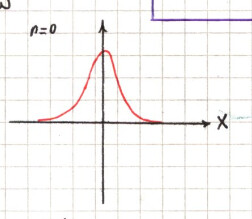
\includegraphics[width=0.35\textwidth]{images/fig_ft2_osc_arm_gaussiana.jpg}

El siguiente estado lo generamos con el operador de creación,
\[
	a^\dagger \Ket{0} = \Ket{1}
\]
de manera que en la pic de abajo podemos ver en la primer fila las funciones de
onda y en la segunda la probabilidad resultante.

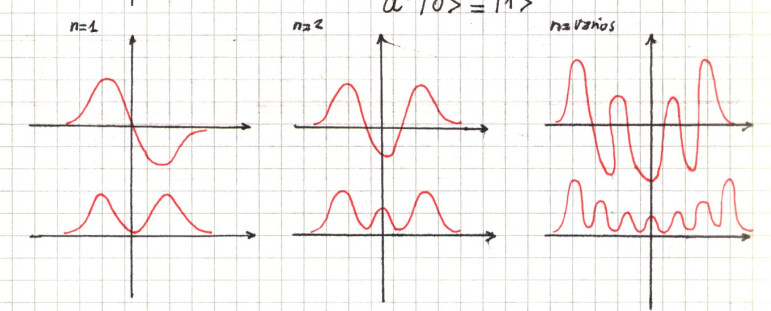
\includegraphics[width=0.9\textwidth]{images/fig_ft2_osc_arm_gaussiana_plancha.jpg}

 
Veamos ahora la evolución temporal en la representación de Heisenberg. Todos los operadores
dependen del tiempo, luego
\[
	\dtot{p}{t} = -\frac{i}{\hbar}[p,H] = -m \omega^2 x \qquad \qquad 
	\dtot{x}{t} = -\frac{i}{\hbar}[x,H] = \frac{p}{m}
\]
y asimismo,
\[
	[p, \frac{p^2}{2m} + \frac{m\omega^2 x^2}{2}] = \frac{m \omega^2}{2} [p,x^2] =
	\frac{m\omega^2}{2}(-2 i \hbar )
\]

Es conveniente hacer una transformación canónica $x,p \to a,a^\dagger$, luego
\[
	\dtot{a}{t} = - i \omega a \qquad \qquad 
	\dtot{a^\dagger}{t} =  i \omega a^\dagger
\]
siendo el conmutador
\[
	[a,H] = \hbar \omega [a,a^\dagger a] = 
	\hbar\omega ( a^\dagger [ a, a ] + [ a, a^\dagger ] a )
\]
con
\[
	a(t) = a(0) \euler^{ - i \omega t } \qquad \qquad 
	a^\dagger(t) = a^\dagger(0) \euler^{ i \omega t }
\]
Poniendo $a,a^\dagger$ en términos de $x, p$ con
\[
	x(t) + i \frac{p(t)}{m\omega} = 
	x(0)\euler^{i\omega t} + i \frac{p(0)}{m\omega}\euler^{-i\omega t}
\]
\[
	x(t) - i \frac{p(t)}{m\omega} = 
	x(0)\euler^{i\omega t} - i \frac{p(0)}{m\omega}\euler^{-i\omega t}
\]
y equating ambas
\[
	x(t) = x(0)\cos(\omega t) + \frac{p(0)}{m\omega} \sin(\omega t)
\]
\[
	p(t) = - m \omega x(0)\sin(\omega t) + p(0) \cos(\omega t).
\]
Esto también se puede calcular con el operador evolución, a través de
\[
	x(t) = \euler^{i H / \hbar t} \: x \: \euler^{-i H / \hbar t},
\]
aunque es un camino mucho más {\it painful}.
Facilitamos un poco con el {\bf lema de Baker-Hausdorff} que dice que
\[
	\euler^{[iG\lambda]} \hat{A} \euler^{-[iG\lambda]} =
	\hat{A} + i \lambda [G,A] + \frac{i^2\lambda^2}{2!}[ G, [G,A ] ] + ... +
	\frac{i^2\lambda^n}{n!} [ G, [ G, [ G, ... [G,A] ] ] ]
\]
con $G$ hermítico y $\lambda$ real.

El primer término es $x$ luego se tienen
\[
	2) \quad [H, x(0)] = - \frac{ i \hbar p(0) }{ m }
\]
\[
	3) \quad [ H, [ H, x(0) ] ] = [ H, -\frac{i \hbar p(0)}{m} ] =
	-[H,p(0)]\frac{i\hbar}{m} = \hbar^2 m x(0)
\]
\[
	4) \quad [ H, [ H, [ H,x(0)] ] ] = [ H, -i \hbar^2 x(0) ] = [ H, x(0) ] \hbar^2
\]
amasando todo esto se llega a
\[
	x(t) = x(0) + \left[ \frac{p(0)}{m} \right] t - \frac{1}{2!}t^2\omega^2 x(0) -
	\frac{1}{3!} \frac{t^3\omega^2 p(0)}{m} + ...
\]
y con un poco de buena vista se pueden identificar en esta serie las expresiones de 
\[
	\sin(\omega t) = \sum_{n=0}^\infty \frac{(\omega t)^{2n+1}}{(2n+1)!} (-1)^n
\]
\[
	\cos(\omega t) = \sum_{n=0}^\infty \frac{(\omega t)^{2n}}{(2n)!} (-1)^n
\]
 
Faltaría ver la evolución de los valores medios $\Braket{n|x(t)|n}=0$ y 
$\Braket{n|p(t)|n} = 0 $, pero se quedan en cero por ser estacionarios [?].
Las oscilaciones solamente aparecerán en estados que son combinación lineal de autoestados
de energía.
 
\end{ejemplo}


\subsection{Interferencia en experimento de Young}

Consideremos la situación depicted en la figura bajo estas líneas, que es reminiscente de la del
experimento de Young aunque la fuente no necesariamente es de luz.

\begin{figure}[h]
	\begin{center}
	\includegraphics[width=0.6\textwidth]{images/teo2_6.pdf}
	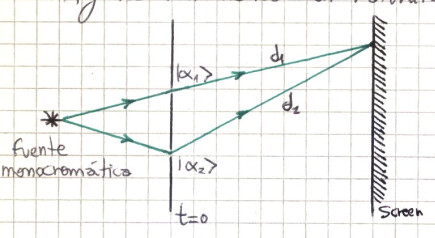
\includegraphics[width=0.6\textwidth]{images/fig_ft2_young_analogous.jpg}
	\end{center}
	\caption{}
\end{figure} 

Uso $\hat{H}$ de partículas libres y que $\Ket{\a}$ es el generado por la fuente.
Suponemos que en $t=0$ al pasar por las aberturas se da
\[
	\frac{1}{2} \Ket{\alpha} = \Ket{\alpha_1} = \Ket{\alpha_2}
\]
y luego para $t>0$ se tiene 
\[
	\Ket{\tilde{\alpha_1}} = \euler^{ -i H t /\hbar } \Ket{\alpha_1} =
		\euler^{ -i E_\alpha t /\hbar } \Ket{\alpha_1}	
\]
\[
	\Ket{\tilde{\alpha_2}} = \euler^{ -i E_\alpha t /\hbar } \Ket{\alpha_2}	
\]

En la pantalla debe verse la interferencia de los dos estados solapados. La diferencia de caminos
es la que genera la interferencia, y usando que los tiempos son $t_i = d_i/v$ se da
\[
	\Ket{\tilde{\alpha}} = \Ket{\tilde{\alpha_1}} + \Ket{\tilde{\alpha_2}} =
		\euler^{ -i E_\alpha \frac{d_1}{v} /\hbar } \Ket{\alpha_1} +
		\euler^{ -i E_\alpha \frac{d_2}{v} /\hbar } \Ket{\alpha_2}	
\]
\[
	\Ket{\tilde{\alpha}} = \frac{1}{2} \euler^{ -i E_\alpha \frac{d_1}{v} /\hbar } 
		\left[ 1 + \euler^{ -i E_\alpha \frac{d_2-d_1}{v} /\hbar } \right] \Ket{\alpha_1}
\]
y si definimos
\[
	\beta=E_\alpha \frac{d_2-d_1}{v} /\hbar,
\]
resulta entonces
\[
	\Braket{\tilde{\alpha}|\tilde{\alpha}} = 
	\frac{1}{4}| 1 +  \euler^{ -i E_\alpha \frac{d_2-d_1}{v} /\hbar } |^2 =
		\frac{1}{4}( (1+\cos\beta)^2 + \sin^2\beta ) =
			\frac{1}{2} + \frac{1}{2}\cos\left( \beta \right).
\]
Esto sería la intensidad si de radiación electromagnética se tratase.

Al partir el estado $\Ket{\alpha_1} $ y volver a unirlo en $\Ket{\alpha_1} + \Ket{\alpha_2}$ vemos una 
intensidad que depende de la diferencia de camino.

\subsection{Cambio de cero del potencial}

Consideramos una partícula sometida a potencial externo.
El potencial es una maquinación matemática conveniente para el concepto más físico de fuerza.
Es un caso particular de cambio de gauge.


En mecánica clásica la física de un problema no se ve afectada por un cambio de gauge.
Si movemos el cero de potencial, la situación física es la misma.
Veamos qué sucede en mecánica cuántica.
\[
	\Ket{\alpha,t,t_0} = \euler^{ -i (p^2/2m + V(x))(t-t_0)/\hbar} \Ket{\alpha,t_0}
\]
\[
	\Ket{\tilde{\alpha},t,t_0} = \euler^{ -i (p^2/2m + V(x) + V_0)(t-t_0)/\hbar} \Ket{\alpha,t_0}
\]
\[
	\Ket{\tilde{\alpha},t,t_0} = \euler^{ -i V_0(t-t_0)/2 }\Ket{\alpha,t,t_0}
\]
y entonces vemos que $\Ket{\tilde{\alpha},t}$ y $\Ket{\alpha,t}$ difieren en una fase, de manera que los 
valores de expectación (las magnitudes físicas) no cambian (con $V_0$ constante).
El efecto fue meter una fase.

Si el potencial es tal que $V_0 = V_0(t)$ entonces
\[
	\Ket{\tilde{\a},t,t_0} = \euler^{ -i \int_{t_1}^{t_2} V(t) dt } \Ket{\a,t,t_0}.
\]


\begin{figure}[htb]
	\begin{center}
	\includegraphics[width=0.6\textwidth]{images/teo2_7.pdf}
	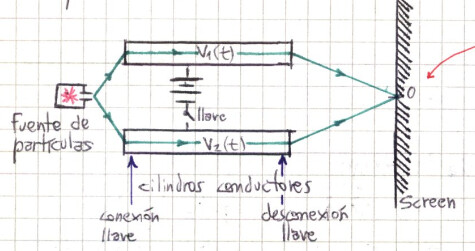
\includegraphics[width=0.6\textwidth]{images/fig_ft2_cero_potential.jpg}
	\end{center}
	\caption{}
\end{figure} 

Consideremos ahora un experimento ideal (pensado). 
Dentro de los cilindros hay campo nulo siempre. Se varia el $V$ abriendo y cerrando la 
llave a la entrada y a la salida; se varía el cero de potencial pero no el campo.
Se cambia la fase de las partículas inferiores respecto de las superiores, entonces habrá interferencia en 
$O$.

Clásicamente no hay variación, pero cuánticamente
\[
	\Delta \text{fase} = -\frac{i}{\hbar}\euler \int _{t_1}^{t_2} V_1(t) - V_2(t) dt = 
	-\frac{i}{\hbar}\euler \Delta V
\]
Notemos que con el límite $\hbar \to 0$ el efecto desaparece [no será el otro límite o hay algo mal?].

Lo que realmente cuenta es la diferencia de potencial $\Delta V$, la cual sí tiene sentido físico porque es 
independiente de la medida y porque pueden escribirse los campos en función de aquella.

\begin{ejemplo}{\bf Caso gravitatorio}
 
Clásicamente la masa inercial con la gravitatoria se cancelan,
\[
	m \ddot{x} = - m \nabla \phi_g
\]
y esto lleva a que la aceleración sea $g$, luego la gravedad es algo geométrico porque no depende de la masa.
Cuánticamente,
\[
	\left( -\frac{\hbar^2}{2m}\nabla^2 + m \phi_g \right) \psi = i \hbar \dpar{\psi}{t}
\]
la masa no se simplifica. Aún así 
\[
	\dtot[2]{}{t} \vm{x} = - g.
\]

 
\end{ejemplo}


\begin{ejemplo}{\bf Experimento Colella/Overhauser/Werner}

Esto viene de un artículo de Physical Review Letters.
Se utilizan partículas neutras: neutrones.
Consideramos el setup siguiente
 
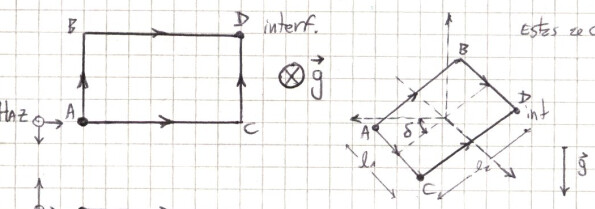
\includegraphics[width=0.6\textwidth]{images/fig_ft2_colella.jpg} 

La diferencia de altura es $\Delta h = \ell_2 \sin \delta $ pero en la derecha se tiene que
$\bar{BD}$ está a mayor altura que $\bar{AC}$ que está más baja.
Luego, la longitud de onda Compton
\[
	v = \frac{p}{m} = \frac{1}{m} \frac{2m\hbar}{\lambda} = \frac{\hbar}{m\lambda_c}
\]
y entonces
\[
	\euler^{ - i/\hbar m g \ell_x \sin \delta \ell_1/v }
\]
de manera que
\[
	\phi_{ABC} - \phi_{ACD} = \frac{ m^2 g \ell_1 \ell_2 \lambda_c \sin \delta }{\hbar^2}
\]
se tiene un fenómeno puramente cuántico (aparece $\hbar$) y depende de la masa.
  
\end{ejemplo}

\subsection{Caso del EM y la invariancia de gauge}

Recordemos algunos resultados del electromagnetismo.
\[
	E = - \Nabla\phi - \frac{1}{c}\dpar{\vb{A}}{t}
\]
Si el cuadrivector de momento es $p^\mu = (E/c, \vb p)$ y el de cuadri potencial es $A^\mu =(\phi,\vb A)$
se veía que el reemplazo
\[
	p^\mu \to p^\mu - \frac{e}{c} A^\mu
\]
era covariante.
Luego, el hamiltoniano covariante era
\be
	H = \frac{1}{2m} \left( \vb{p} - \frac{\euler\vb{A}}{c}\right)^2 + \euler \phi 
	\label{ham_cov_em}
\ee

En el formalismo de Heisenberg
\[
	\dtot{H}{t} = \frac{1}{i\hbar}[x_i,H] = \frac{p_i - e A_i / c}{m}
\]
puesto que $p$ y $A$ no conmutan. Los momentos son justamente $\pi_i = p_i - e/c A_i$.
Luego,
\[
	[ p_i, p_j ] = 0 \qquad 
	[ \pi_i , \pi_j ] = \frac{i\hbar e}{c} \epsilon_{i l k}B_k
\]

La invariancia de gauge hace que
\[
	\phi \to \phi - \frac{1}{c}\dpar{\Lambda}{t} \qquad \quad 
	\vb A \to \vb A + \nabla \Lambda
\]
que es un cambio que deja los campos $\vb E, \vb B$ invariantes. Si la función $\Lambda \neq \Lambda(\vb x)$
entonces el cambio es como un cambio de cero del potencial, pues 
\[
	\phi \to \phi + \lambda(t) \qquad \vb A \to \vb A.
\]

La mecánica cuántica incluye la invariancia de gauge de modo que los valroes de expectación, que es lo
físico, no se alteran.
El cambio de fase implicado por la transformación de gauge no pasa a los valores de expectación.

Considerando la versión operacional del hamiltoniano \eqref{ham_cov_em} y la ecuación de Schrödinger,
\[
	H \Ket{\a,t_0,t} = i \hbar \dpar{}{t} \Ket{\a,t_0,t}
\]
Ahora quiero hacer una transformación de gauge para ver si obtengo las mismas mediciones.
Reemplazando los operadores $p$ y $A$ por los transformados según el cambio de gauge se obtiene
(luego veremos la justificación, creámoslo por ahora)
\[
	\Ket{\tilde{\a},t_0,t} = \euler^{ i e \Lambda(x,t)/(\hbar c)}\Ket{\a,t_0,t} 
\]
y a esta fase la denominaresmos $\hat{g}(x,t)$ (un operador?) luego, la transformación de gauge implica
\[
	\Braket{\a|x|\a} \to  \Braket{\tilde{\a}|x|\tilde{\a}} = \Braket{\a|g^\dagger x g|\a}
\]
y como conmutan,
\[
	\Braket{\a|x g^\dagger g|\a} = \Braket{\a|x|\a}
\]
donde el último paso es por la unitariedad. Luego, el $x$ no cambia por una transformación de gauge.

Veamos qué le pasa al momento conjugado $\pi$, teniendo en cuenta que el momento lineal mecánico $p$ no varía
pero sí el potencial $A$, i.e.
\[
	\Braket{\a|\pi|\a} \to  \Braket{\tilde{\a}|\tilde{\pi}|\tilde{\a}} =
	\Braket{\tilde{\a}| p - \frac{e\tilde{A}}{c} |\tilde{\a}}
\]
Luego,
\[
	\Braket{\tilde{\a}| g^\dagger \left( p - \frac{e {A}}{c} - \frac{e}{c} \nabla\Lambda \right) g |\tilde{\a}}
\]
donde hay que recordar que $p$ tiene metida la derivada respecto de $x$ y $A, \Lambda$ son sólo dependientes
de $x,t$ y conmutan con $g(x,t)$. Se ve que resulta todo el operador $p - e/c A$ y la transformación cumple
además que $\Braket{\a|\a} =  \Braket{\tilde{\a}|\tilde{\a}} $ de forma que se ha demostrado lo que se
propusiera antes.
Tenemos
\begin{multline}
	\left[ \frac{1}{2m}\left( p - \frac{e {A}}{c} - \frac{e \nabla\Lambda}{c} \right)^2 +
	e \: \phi - \frac{e}{c} \dpar{\Lambda}{t} \right] 
	\euler^{i e \Lambda/ (\hbar c)} \Ket{\a,t_0,t} = \\
	\euler^{i e \Lambda/ (\hbar c)} 
	\left( - \frac{e}{c} \dpar{\Lambda}{t} + i \hbar \dpar{}{t} \right) \Ket{\a,t_0,t}
\end{multline}
donde se ve que valen varias cosas
\[
	g g^\dagger \left( p - \frac{e {A}}{c} - \frac{e \nabla\Lambda}{c} \right) g = 
	g \left( p - \frac{e {A}}{c}  \right)
\]
Con esto debería ser suficiente para confirmar el resultado [confirmarlo].
La mecánica cuántica es, entonces, invaraitne de gauge al igual que lo que sucedía en mecánica clásica.

\begin{ejemplo}{\bf Experimento de Aharonov y Bohm}

Vemos en la figura que las partículas no interactúan con el campo $\vb B$ y el circulito es un solenoide
infinito. Hay campo magnético dentro pero es nula afuera. Tengo, no obstante, potencial $\vb A$ en todas
partes.

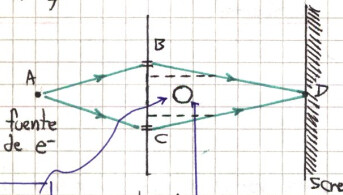
\includegraphics[width=0.5\textwidth]{images/fig_ft2_aharonov_bohm.jpg} 

Luego, resulta que hay interferencia en $D$ sin campo $\vb B$ por al diferencia de fases originada por el potencial
$\vb A$.

La fase es
\[
	- \frac{i}{\hbar} \int_{t_1}^{t_2} \left( - \frac{e}{c} \dtot{\vb x}{t} \cdot \vb A\right) dt=
	\frac{i e}{\hbar c} \int_{x_1}^{x_2} \vb A \cdot d\vb x.
\]
Recordemos que el lagrangiano de la situación\footnote{Hay un lagrangiano para cada momento, como para ahora
que me estoy tomando una copa de vino.} [?]
\[
	\Lag = \frac{m}{2} \Dtot{\vb x}{t}^2 + \frac{e}{c} \dtot{\vb x}{t}\cdot\vb A
\]

Quisiéramos ver cuál es la diferencia de fase entre los dos caminos ABD y ACD, que será
\[
	\frac{ie}{\hbar c} \left( \int_{ABD} \vb A\cdot d\vb x - \int_{ACD} \vb A\cdot d\vb x \right) =
	\frac{ie}{\hbar c} \left( \int_{ABD} \vb A\cdot d\vb x + \int_{DCA} \vb A\cdot d\vb x \right) =
	\frac{ie}{\hbar c}  \int_{cerrada} \vb A\cdot d\vb x
\]
que conduce a
\[
	\frac{ie}{\hbar c}  \int_{cerrada} \rotorm{A} \: d\vb S = \frac{ie}{\hbar c} \phi_B \neq 0
\]
es decir que hay efecto de interferencia. Notemos que el rotor sigue siendo invariante de gauge [?].

Físicamente el campo $\vb B$ no interactúa con el ahz de partículas, con lo cual parecería una interacción
del potencial con las partículas.
 
\end{ejemplo}


% =================================================================================================
\section{El propagador}
% =================================================================================================

Físicamente representa la proababilidad de transición entre autoestados por el paso del tiempo,
$ \Ket{x'}_{t_0} \longrightarrow \Ket{x''}_t$
\[
	\Braket{x''|\euler^{-iH(t-t_0)/\hbar}|x'} \equiv K(x',t; x, t_0)
\]
\[
	\Braket{x''| \alpha,t_0,t} = \Braket{x''|\euler^{-iH(t-t_0)/\hbar}|\alpha,t_0} 
\]
\[
	\Braket{x''| \alpha,t_0,t} = \int dx' \Braket{x''|\euler^{-iH(t-t_0)/\hbar}|x'}\Braket{x'|\alpha,t_0} 
\]
\[
	\Psi_{\alpha}(x'',t) = \int dx' K(x'',t; x',t) \Psi_{\alpha}(x',t)
\]

Podemos pensar que el propagador lleva la función de onda desde $t_0$ a $t$. Se puede escribir:
\[
	K(x',t; x, t_0) = \sum_{a'} \Braket{x''|a'} \Braket{a'|x'} \euler^{-iE_a(t-t_0)/\hbar}
\]
y metemos un observable $\hat{A}$ donde $[A,H]=0$ y $A\Ket{a'}=a\Ket{a'}$.

El propagador depende del potencial, pero no de la función de onda inicial. Se debe cumplir que:
\[
	\lim_{t\to t_0} K(x',t; x, t_0) = \delta^3(x''-x')
\]
\[
	K(x'',t; x, t_0) = \Braket{x''|\euler^{-iH(t-t_0)/\hbar}|a'} \Braket{a'|x'} =
		\sum_{a'} \Psi_{\Ket{a'}}(x'',t)\Braket{a'|x'}
\]
\[
	K(x'',t; x, t_0) = \sum_{a'} c_{a'}(x')\Psi_{\Ket{a'}}(x'',t)
\]
y entonces el propagador es una función de Green que satisface 
\[
	\left( -\frac{\hbar^2}{2m}\nabla^2 +V(x'') - i\hbar\dpar{}{t} \right)K(x',t; x, t_0) =
		- i\hbar \delta^3(x''-x') \delta(t-t_0)
\]
con $K(x'',t;x',t_0)=0 $ si $t<0$ que es la condición de contorno.

\subsection{El propagador de la partícula libre}

\[
	K(x'',t; x, t_0) = \int dp' \Braket{x''|\euler^{-ip^2(t-t_0)/2m\hbar}|p'} \Braket{p'|x'} 
\]
\[
	= \int dp' \euler^{-ip'^{2}(t-t_0)/2m\hbar} \Braket{x''|p'} \Braket{p'|x'} =
	\frac{1}{2\pi\hbar} \int dp' \euler^{-ip'^{2}(t-t_0)/2m\hbar} \euler^{-ip'(x'-x'')/\hbar}
\]
y entonces el propagador de una partícula libre es
\[
	K(x'',t; x, t_0) = \sqrt{ \frac{m}{2\pi\hbar(t-t_0)} } \euler^{i\frac{m(x''-x')^2}{2\hbar(t-t_0)}}
\]

También se puede escribir el propagador en la representación de Heisenberg,
\[
	\Braket{x''|\euler^{-iH(t-t_0)/\hbar}|x'} = \Bra{x''}\euler^{-iHt/\hbar} \euler^{iHt_0/\hbar}\Ket{x'}=
		\Braket{x'',t|x',t_0}
\]
\[
	K(x'',t;x',t_0) = \Braket{x'',t | x',t_0}.
\]

El propagador cumple con la propiedad de composición (como el $U(t,t_0)$), es decir:
\[
	K(x'',t; x, t_0) = K(x'',t; x, t_1)K(x'',t_1; x, t_0) \qquad t>t_1>t_0
\]

% =================================================================================================
\section{Integrales de camino de Feynmann}
% =================================================================================================

Consideramos una partícula yendo de $(x_1,t_1)$ a $(x_N,t_N)$. Dividimos el tiempo 
\[
	\delta t = \frac{t_N-t_1}{(N-1)}
\]
y queremos ver la amplitud de transición desde el estado 1 al $N$.

\begin{figure}[htb]
	\begin{center}
	\includegraphics[width=0.6\textwidth]{images/teo2_8.pdf}	 
	\end{center}
	\caption{}
\end{figure} 

\[
	\braket{x_N,t_N|x_1,t_1} = \int dx_{N-1}\int dx_{N-2} \; ...\int dx_2
	\Braket{x_N,t_N|x_{N-1},t_{N-1}} ...\Braket{x_2,t_2|x_1,t_1}
\]

Se puede pensar como que estamos sumando sobre todos los posibles caminos entre $(x_1,t_1)$ y $(x_N,t_N)$ 
fijos. En mecánica clásica teníamos un solo camino, el que minimizaba la acción $S$
\[
	\delta \int_{t_1}^{t_2} \Lag dt = \delta S = 0
\]
pero en cambio en mecánica cuántica todos los caminos aportan. En un libro de Dirac, Feymann lee 
\[
	\Braket{x_2,t_2|x_1,t_1} \; \text{corresponde a} \; \euler^{i\int_{t_1}^{t_2}\Lag/\hbar dt}
\]
Definiremos
\[
	S_{(n,n-1)}\equiv \int_{t_{n-1}}^{t_n}\Lag(x,\dot{x}) dt
\]
Luego para considerar la suma sobre todos los segmentillos a lo largo de un camino tendremos
\[
	\prod_{n=2}^N \euler^{i/\hbar S(n,n-1)} = \euler^{i/\hbar \prod_{n=2}^N S(n,n-1)} = \euler^{iS(N,1)/\hbar}
\]
y hay que considerar TODOS los posibles caminos 
\[
	\propto \sum_{caminos} \euler^{i/\hbar S(N,1)} 
\]
cuando $\hbar \to 0$ las trayectorias contribuyen con una cantidad que oscila loca y violentamente. Tienden a 
la cancelación para caminos aledaños. Por el $\hbar \sim 0$ la fase es grande y entonces se cancelan.
Esto no ocurre cerca del camino (real) que cumple 
\[
	\delta S(N,1) = 0
\]
Para trayectorias cercanas la $\Delta fase$ no es grande y hay interferencia constructiva.
Para un $\delta t$ infinitesimal es 
\[
	\Braket{x_n,t_n|x_{n-1},t_{n-1}} = N \euler^{iS(n,n-1)/\hbar}
\]
\[
	S(n,n-1) = \int_{t_{n-1}}^{t_n} \left( \frac{m}{2}\dot{x}^2 - V(x)\right) dt \approx
	\int_{t_{n-1}}^{t_n} \left( \frac{m}{2} \frac{(x_n-x_{n-1})^2}{\delta t^2} - 
	V\left(\frac{x_n+x_{n-1}}{2}\right)\right)  dt
\]
donde la última expresión es a orden 1 (pues $\delta t \sim 0$).
\begin{figure}[htb]
	\begin{center}
	\includegraphics[width=0.6\textwidth]{images/teo2_9.pdf}
	\end{center}
	\caption{}
\end{figure} 

Consideremos, por ejemplo, una partícula libre, entonces $V=0$ de modo que resolviendo 
\[
	\Braket{x_n,t_n|x_{n-1},t_{n-1}} = N \euler^{im(x_n - x_{n-1})/2\hbar\delta t}
\]
Esto no es otra cosa que el propagador de una partícula libre. Para un $\Delta t$ finito será 
\[
	\Braket{x_n,t_n|x_1,t_1}  = \lim_{N\to\infty} \left(\frac{m}{i2\pi\hbar\delta t}\right)^{(N-1)/2}
	\int dx_{n-1}\int dx_{n-2} \; ... \int dx_2 \prod_{n=2}^N \euler^{i S(n,n-1)/\hbar}
\]
\[
	\Braket{x_n,t_n|x_1,t_1}  = \int_{x_1}^{x_n} D[x(t)] \euler^{i \int _{t_1}^{t_n} \Lag(x,\dot{x})/\hbar} dt
\]
siendo esta última la integral de camino de Feynmann.

En base a éstas Feynamn desarrolla una formulación equivalente de la mecánica cuántica que utiliza los 
conceptos de:
\begin{enumerate}
 \item Superposición
 \item Composición de la transición
 \item Límite clásico con $\hbar \to 0$
\end{enumerate}

Estas integrales contienen toda la información del sistema cuántico, aunque no sea sencillo extraerla.

Consideremos un propagador de $(x',0) \to (x',t)$
\[
	G(t) = \int dx' K(x',t ; x', 0) = \int dx' \Braket{x'|\euler^{-i Ht/\hbar}|x'}
\]
\[
	G(t) = \sum_{a'} \int dx' \Braket{x'|\euler^{-i Ht/\hbar}|a'}\Braket{a'|x'} =
		\sum_{a'} \euler^{-i E_{a'}t/\hbar} \int dx' \Braket{x'|a'}\Braket{a'|x' }
\]
\[
	G(t) = \sum_{a'} \euler^{-i E_{a'}t/\hbar} \int dx' |\Braket{x'|a'}|^2 = \sum_{a'} \euler^{-i E_{a'}t/\hbar} 
\]
que es reminiscencia de la función de partición de mecánica estadística. Tomando Laplace-Fourier 
\[
	\tilde{G}(E) = -i \int dE \frac{G(t)}{\hbar} \euler^{i E t/\hbar} = \sum_{a'} \frac{1}{E-E_{a'}}
\]
y el espectro de autoenergías son los polos de $\tilde{G}(E)$.

La expresión 
\[
	\Braket{x,t|x_1,t_1} \equiv \text{Integral de camino de Feynmann}
\]
satisface la ecuación de Schrödinger y es una alternativa a la formulación de la cuántica usual.


% \bibliographystyle{CBFT-apa-good}	% (uses file "apa-good.bst")
% \bibliography{CBFT.Referencias} % La base de datos bibliográfica

\end{document}
